\documentclass{article}
\usepackage{graphicx, physics, dsfont}
\usepackage{fancyhdr}
\usepackage{hyperref}
\usepackage{ragged2e}
\usepackage{amsmath, amsthm, amssymb}
\usepackage[margin=1in]{geometry}
\usepackage{setspace}
\usepackage{tikz}
\usetikzlibrary{positioning}

\pagestyle{fancy}
\lhead{Zoeb Izzi}
\rhead{\today}
\lfoot{Problem Set 1}
\rfoot{}

\begin{document}
    \thispagestyle{fancy}
    \begin{center}
                \LARGE{Complex Analysis \\ Problem Set 1}
    \end{center}
    \vspace{10mm}
    In problems 1-8, give a clear geometric description of the set of complex points satisfying the given relation.
    \begin{enumerate}
        \item $|z + 4| = 7$ represents a circle centered at $-4$ with radius $7$.
        \item $|z - i| < 2$ represents the interior of a circle (excluding the boundary) centered at $i$ with radius $2$.
        \item $4 < |z - 2i| \le 6$ represents the region between the two concentric circles centered at $2i$ with radii $4$ and $6$, including the boundary of the outer circle and excluding the boundary of the inner circle.
        \item $|z + 2| = |z - i|$ represents the perpendicular bisector of the segment connecting $-2$ and $i$.
        \item $|z - 2| + |z + 3i| = 5$ represents an ellipse with foci at $2$ and $-3i$, with its major axis being a line segment of length $5$.
        \item $|z + 3| - |z - 1| = 2$ represents one branch of a hyperbola with foci at $-3$ and $1$, where the difference of distances to the foci is always 2.
        \item $|z + 2| = \Re(z) + 3$ represents a parabola with vertex at $-2.5$ and opening to the right, where the distance from any point on the parabola to the focus at $-2$ is equal to the distance from that point to the directrix at $x = -3$.
        \item $|\Re(z)| > 2$ represents the entire complex plane except the region with real component between $-2 \le \Re(z) \le 2$, a vertical strip.
    \end{enumerate}
In problems 9-14, determine the image of the number $z = 1 + 2i$ under the given function and explain in your own words what the transformation does to this number. Graph both the point and its image on the complex plane.
\begin{enumerate}\setcounter{enumi}{8}
        \item $f(z) = 3z$ images the point $z = 1 + 2i$ to $z = 3+6i$. This transformation scales the point by a factor of 3 away from the origin,  stretching the distance from the origin while maintaining the same angle.
        \item $f(z) = iz$ images the point $z = 1 + 2i$ to $z = -2 + i$. This transformation rotates the point $90^\circ$ counterclockwise about the origin.
        \item $f(z) = z + 1 - 3i$ images the point $z = 1 + 2i$ to $z = 2 - i$. This transformation translates the point by adding $1 - 3i$ to it.
        \item $f(z) = (1+i)z$ images the point $z = 1 + 2i$ to $z = -1 + 3i$. This transformation scales the point by a factor of $\sqrt{2}$ and rotates it by $45^\circ$ counterclockwise about the origin.
        \item $f(z) = z^2$ images the point $z = 1 + 2i$ to $z = -3 + 4i$. This transformation squares the complex number, which results in a rotation and scaling of the point in the complex plane, squaring the modulus and doubling the argument of any given complex number.
        \item $f(z) = \frac{1}{z}$ images the point $z = 1 + 2i$ to $z = \frac{1}{1 + 2i} = \frac{1 - 2i}{5} = \frac{1}{5} - \frac{2}{5}i$. This transformation takes the reciprocal of the complex number, which reflects the point across the real axis and inverts its distance from the origin.
    \end{enumerate}
    \newpage
\vspace{5mm}
\noindent Below is the complex plane illustrating the original point $z = 1+2i$ and its images under the transformations $f(z)$ in problems 9 through 14. 

\vspace{10mm}

\begin{center}
    % The scale=1.4 makes the graph huge so it takes up a good portion of the page.
    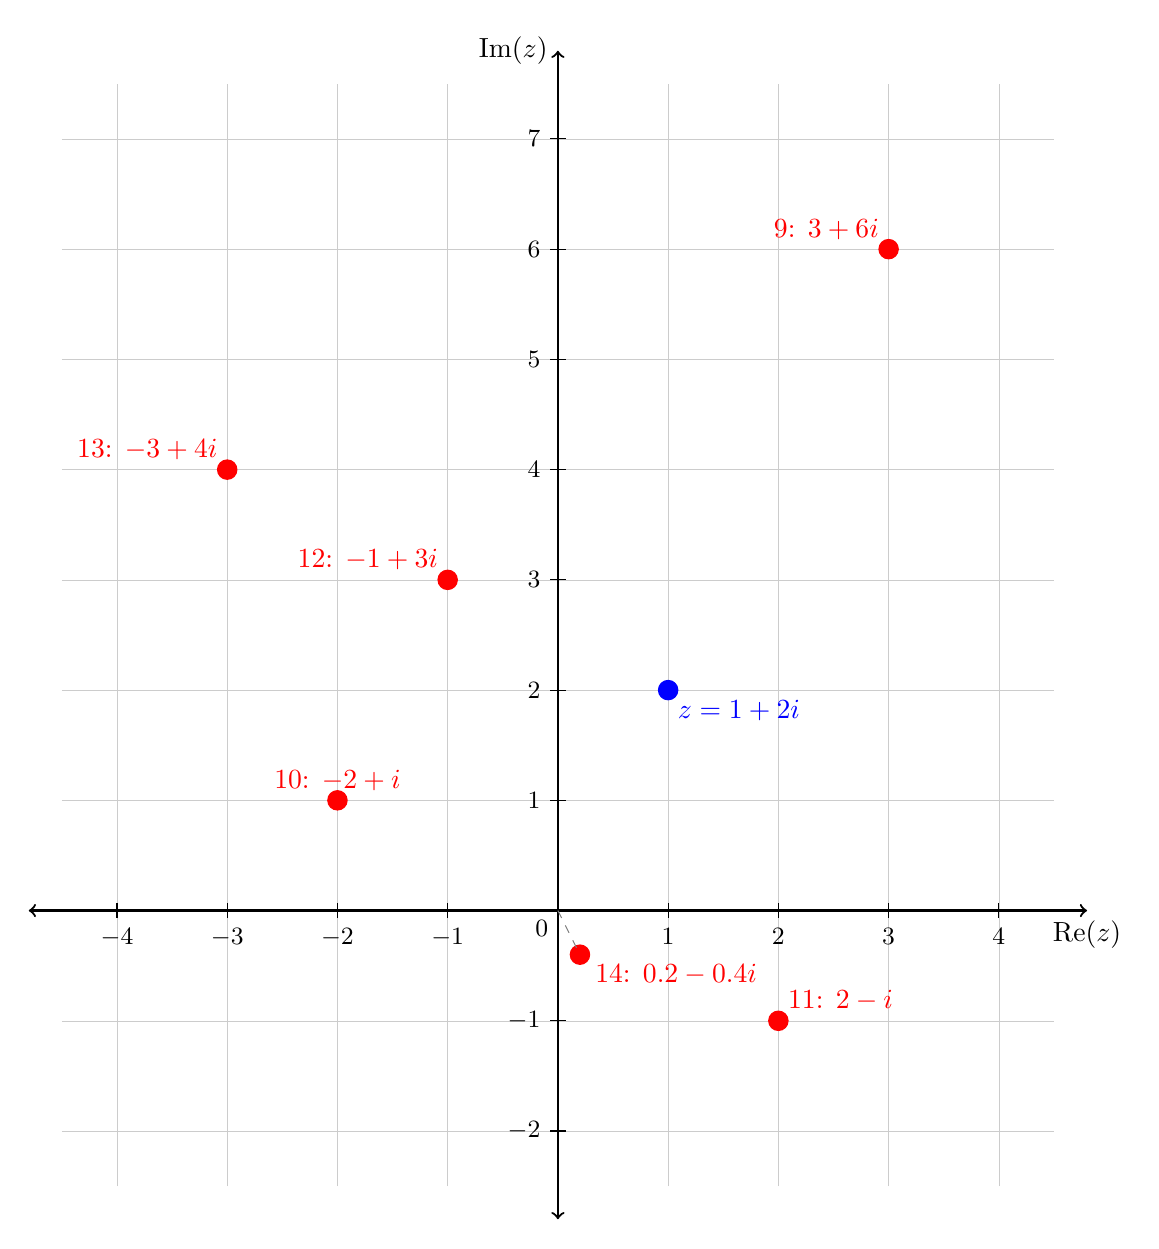
\begin{tikzpicture}[scale=1.4]
        
        % Draw grid
        \draw[step=1cm, gray!40, very thin] (-4.5, -2.5) grid (4.5, 7.5);
        
        % Draw axes
        \draw[thick, <->] (-4.8, 0) -- (4.8, 0) node[anchor=north] {$\Re(z)$};
        \draw[thick, <->] (0, -2.8) -- (0, 7.8) node[anchor=east] {$\Im(z)$};
        
        % X-axis ticks
        \foreach \x in {-4,-3,-2,-1,1,2,3,4}
            \draw (\x, 2pt) -- (\x, -2pt) node[anchor=north] {\small $\x$};
            
        % Y-axis ticks
        \foreach \y in {-2,-1,1,2,3,4,5,6,7}
            \draw (2pt, \y) -- (-2pt, \y) node[anchor=east] {\small $\y$};
            
        % Origin label
        \node[anchor=north east] at (0,0) {\small $0$};

        % Original Point z (Blue)
        \filldraw[blue] (1,2) circle (2.5pt) node[anchor=north west] {$z = 1+2i$};
        
        % Mapped Points (Red)
        % 9: f(z) = 3z
        \filldraw[red] (3,6) circle (2.5pt) node[anchor=south east] {9: $3+6i$};
        
        % 10: f(z) = iz
        \filldraw[red] (-2,1) circle (2.5pt) node[anchor=south] {10: $-2+i$};
        
        % 11: f(z) = z + 1 - 3i
        \filldraw[red] (2,-1) circle (2.5pt) node[anchor=south west] {11: $2-i$};
        
        % 12: f(z) = (1+i)z
        \filldraw[red] (-1,3) circle (2.5pt) node[anchor=south east] {12: $-1+3i$};
        
        % 13: f(z) = z^2
        \filldraw[red] (-3,4) circle (2.5pt) node[anchor=south east] {13: $-3+4i$};
        
        % 14: f(z) = 1/z
        \filldraw[red] (0.2,-0.4) circle (2.5pt) node[anchor=north west, xshift=2pt] {14: $0.2-0.4i$};
        
        % Draw dashed line to 1/z just to help it stand out near the origin
        \draw[dashed, gray] (0,0) -- (0.2,-0.4);
        
    \end{tikzpicture}
\end{center}
\end{document}
